\section{Requirements} \label{sec:Requirements}

\subsection{Business Case} \label{sec:Requirements.BusinessCase}
Any personal accounting system should be able to provide accurate and relevant
summaries of an individual's financial status. In order to do this, the user
needs to be able to supply the system with the necessary data, so that it can
be analysed and properly converted into knowledge.

It seems fair to infer that nowadays most of a user's financial transactions
happen in ways that can be listed electronically (usually via their bank or
credit card statements) -- a study by Payments UK
(\citeyear{paymentsUK2017summary}), for example, indicates that there has been
a rise in debit card payments over the past few years, and that the volumes of
this type of transaction is likely to be higher than that of cash payments by
the year 2021. Therefore, an assumption has been made that the users will
require means of uploading a list of their financial transactions into the
system.

The system created for this project intends to do just this. Its main feature,
however, will be to allow the user to categorise expenditure based on patterns
in the entries' descriptions. There must also be a feature to allow the user to
view summaries of the income and expenditure over a period of time, as well as
one to forecast budgets for future periods based on the ``financial behaviour''
analysed.

A feature to estimate tax would also be useful. Initially, this can be based on
the system used to calculate personal tax in the UK, where all of an
individual's income is added up, and depending on which threshold it reaches,
tax is deducted at that level. For example, for an individual earning
\pounds75,000 per annum from their job where he or she is a company employee,
initially their tax free allowance would be deducted from the gross figure,
then the basic rate is deducted from it up to its limit, then higher rate would
be deducted from the rest. However, if they have any income from sources which
have special taxation rules, such as interest on savings, these would be
deducted right after the personal allowance -- that is, income from special
taxation sources get added to the gross income figure, but tax from them is
deducted at a different rate and before the base tax. (\textbf{TODO: CITATION
NEEDED}).

There should be an option to allow a user to determine whether a transaction is
taxable. For income, the user should also be able to determine if it is already
net of tax (taxed at source) or if it's the gross amount, since this would
influence the tax calculation. Also, on expenditure, certain costs such as
memberships to professional organisations are deductible, so the user should be
able to indicate this when they are registering the category.

Furthermore, for the tax feature, it is important to emphasise that not all of
an individual's income will get taxed under income tax. For example, profits on
sales of shares gets taxed as capital gains tax. Since this type of tax is
outside of the scope of this application but would still appear on a user's
list of transactions, the system needs a way to highlight these so as for them
not to be included in the tax calculation.



\subsection{Functional Requirements} \label{sec:Requirements.FunctionalRequirements}

Based on the description above, a few functional requirements were identified.
They are represented in the diagram on section
\ref{sec:Requirements.FunctionalRequirements.UseCaseDiagram} and the list,
wireframes and activity diagrams on section
\ref{sec:Requirements.FunctionalRequirements.UseCaseList}.

\subsubsection{Use Case Diagram} \label{sec:Requirements.FunctionalRequirements.UseCaseDiagram}
Use case diagrams are UML constructs which were developed by Jacobson et al.
(1992, cited \cite[][p.~154]{bennett2010object}). The use case diagram on
Figure \ref{fig:UseCaseDiagram} is used to illustrate the functional
requirements identified for this project:
\begin{figure}[ht!]
  \begin{center}
    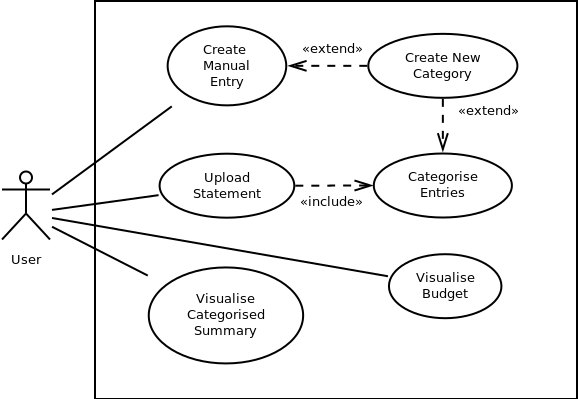
\includegraphics[width=14cm]{./contents/img/Use_Case_Diagram.png}
  \end{center}
  \caption{Use Case Diagram}
  \label{fig:UseCaseDiagram}
\end{figure}
\FloatBarrier



\subsubsection{Use Case List} \label{sec:Requirements.FunctionalRequirements.UseCaseList}
Table \ref{tab:UseCaseDescriptions} lists the descriptions for the use cases
listed above:
\begin{table}[ht!]
  \centering
  \begin{tabular}{|p{4cm}|p{12cm}|}
    \hline
    \textbf{Use Case}&\textbf{Description}\\
    \hline
    Upload Statement&The user must be able to upload a list of their
                     financial transactions, most likely their bank
                     or credit card statements, in a valid format, and all
                     entries should be categorised based on specific patterns\\
                    &\emph{Includes}: Categorise Entries\\
    \hline
    Create Manual Entry&The user should be able to create a manual transaction for
                        income or expenditure, include a date, amount and
                        description, and either choose an existing category (or
                        categories) for it or create a new one(s) in the
                        process\\
                        &\emph{Extends}: Create Category\\
    \hline
    Visualise Categorised Summary&The user must be able to visualise
                                  a summary of their income and expenditure
                                  over a period of time\\
    \hline
    Calculate Budget&The user must be able to visualise a budget for future
                     periods based on their income and expenditure data 
                     already entered\\
    \hline
    Categorise Items&Analyse the current entry and assign it to a category\\
                    &\emph{Extends}: Create Category\\
    \hline
    Create Category&Creates a new category with the name suggested by the
                        user\\
    \hline
    Estimate Tax&Based on the information entered and the current tax year,
                 calculate how much tax is due\\
    \hline
  \end{tabular}
  \caption{Use Case Descriptions} \label{tab:UseCaseDescriptions}
\end{table}
\FloatBarrier

The wireframe below (Figure \ref{fig:Wireframe.CreateManualEntry}) was created
to better illustrate the \emph{Manual Entry} requirement from the point of view
of the user. It shows an example of an entry for a laptop and a licence for a
proprietary operating system, which can then be broken down among different
categories. The user has the option to use the percentage or the amount boxes
in order to provide a breakdown, and they can also add new lines if more than
one is required -- the example shows two lines, but the default would be one.
Under the category search box, if the user types a category name that does not
exist they will be asked if they want to create a new one:
\begin{figure}[ht!]
  \begin{center}
    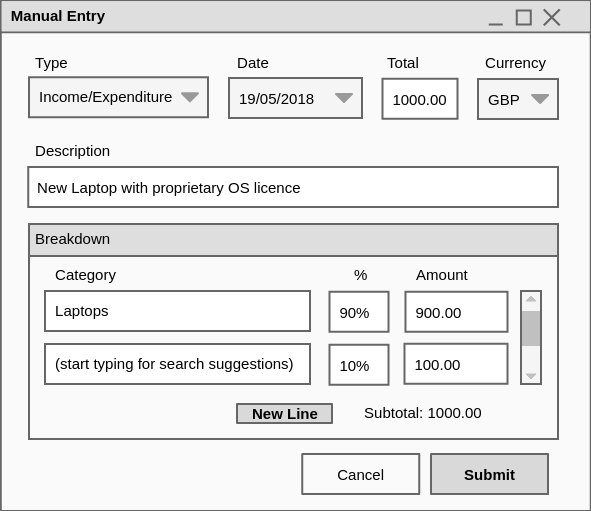
\includegraphics[width=14cm]{./contents/img/Wireframe_-_Manual_Entry.png}
  \end{center}
  \caption{User interface wireframe for \emph{Create Manual Entry} use case}
  \label{fig:Wireframe.CreateManualEntry}
\end{figure}
\FloatBarrier

And in order to better understand the relationship between \emph{Upload
Statement} and \emph{Categorise Entries}, the activity diagram below (Figure
\ref{fig:AD.CategoriseEntries}) was developed:
\begin{figure}[ht!]
  \begin{center}
    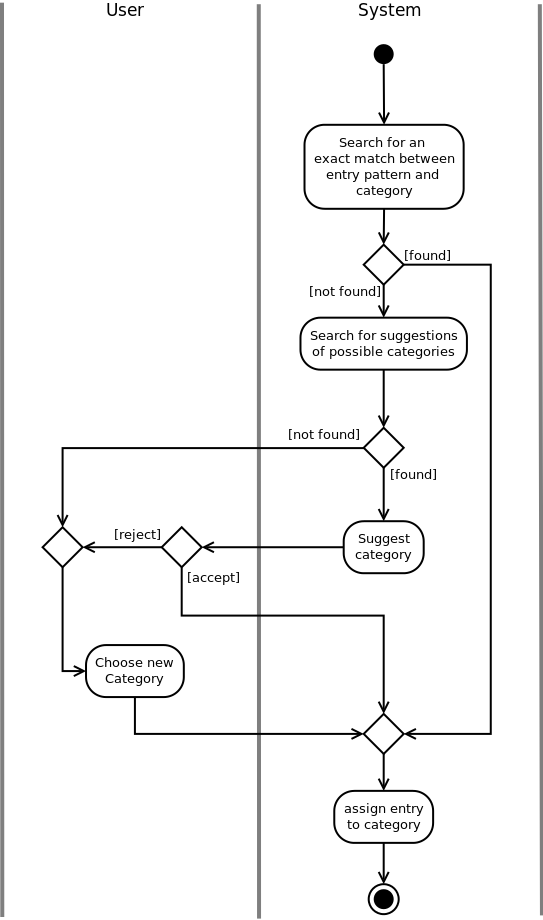
\includegraphics[width=11cm]{./contents/img/Activity_Diagram_-_Categorise_Entries.png}
  \end{center}
  \caption{}
  \label{fig:AD.CategoriseEntries}
\end{figure}
\FloatBarrier

Below (Figure \ref{fig:Wireframe.VisualiseCategorisedSummary}) is also a
wireframe illustrating the GUI for \emph{Visualise Categorised Summary}. The
user should have an option to select the dates and, if they only want to see
one category, the category itself:
\begin{figure}[ht!]
  \begin{center}
    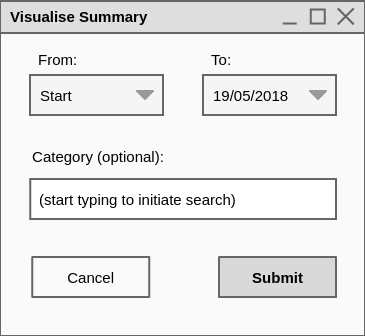
\includegraphics[width=8cm]{./contents/img/Wireframe_-_Visualise_Summary.png}
  \end{center}
  \caption{}
  \label{fig:Wireframe.VisualiseCategorisedSummary}
\end{figure}
\FloatBarrier

The dates field should allow them both to type a date or choose it from a drop
down calendar. If no values are entered, the system will return a summary of
all categories on the system.



Below is a wireframe to illustrate how the initial window for the
\emph{Estimate Tax} requirement:

\textbf{TODO}

\begin{figure}[ht!]
  \begin{center}
    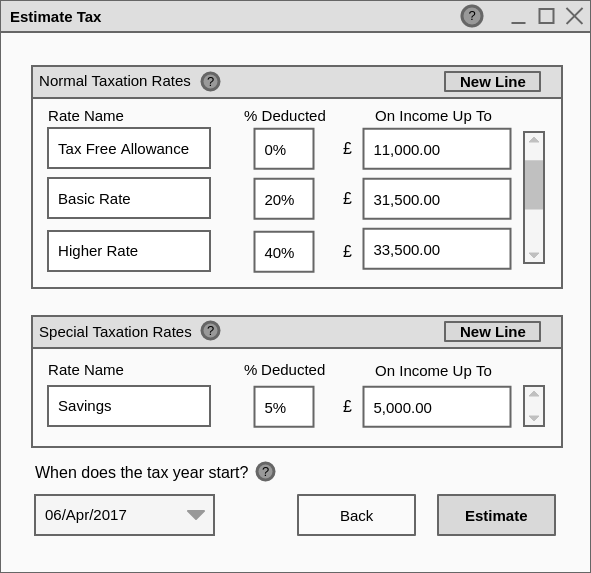
\includegraphics[width=14cm]{./contents/img/Wireframe_-_Estimate_Tax.png}
  \end{center}
  \caption{Estimate Tax interface. Date and allowances shown as specified by HM
    Revenue \& Customs (\cite[][]{hmrc2018taxrates})}
  \label{fig:Wireframe.EstimateTax}
\end{figure}
\FloatBarrier

Normally, in the UK there is a difference between what is ``tax exempt'' and
what is ``taxed at 0\%''.  For the purposes of the estimation provided by
the requirements in this project, it was initially decided that this
distinction would be ignored, and that the user could simply have a choice to
use one of the dynamic boxes on \emph{Normal Taxation Rates} to indicate a tax
free allowance. However, due to the order in which the taxes are to be
deducted, it was decided that a non-taxable allowance field should still be
made available, but allow its value to be set to zero. This should allow for
more flexibility.

The interface would start with one line item, and then more items could be
added if the end user needs them. Each line represents one of the tax rates and
the threshold of income which needs to be reached before it starts deducting
tax at that percentage.

A choice has been made to include help texts next to the fields which are
likely to need them, and these are indicated in Figure
\ref{fig:Wireframe.EstimateTax} by the bubbles with the question marks next to
the relevant fields.

\subsection{Non-Functional Requirements} \label{sec:Requirements.NonFunctionalRequirements}
Use cases and use case diagrams are an appropriate tool to document functional
requirements, but not non-functional ones (Jacobson et al., 1999,
\cite[cited][p.~153]{bennett2010object}). Therefore, a separate list has been
kept in order to document the non-functional requirements, where they exist.
% TODO: make sure I've actually got a list once I understand what these
% requirements are
